\documentclass{article}[12pt]
\usepackage[utf8]{inputenc}
\usepackage{amssymb}
\usepackage{mathtools}
\usepackage{multirow}
\usepackage{textcomp}
\usepackage[a4paper, margin=1 in]{geometry}
\usepackage{graphicx}
\usepackage{hyperref}
\usepackage{bm}
\usepackage{xcolor}
\definecolor{LightGray}{gray}{0.9}
\usepackage{float}
\usepackage{mathrsfs}
\usepackage{natbib}
\usepackage{longtable}
\bibliographystyle{plainnat}
\usepackage{theorem}
\newcounter{theorem}
\renewcommand\thetheorem{\arbic{theorem}}
\newtheorem{theorem}{Theorem}%[theorem]
%\newtheorem{algorithm}{Algorithm}%[theorem]
\newtheorem{corollary}{Corollary}%[section]%[theorem]
\newtheorem{fact}{Fact}%[section]
\newtheorem{property}{Property}%[section]
\newtheorem{result}{Result}%[section]
\newtheorem{lemma}{Lemma}%[section]
\newtheorem{proposition}{Proposition}
%\newtheorem{proof}{Proof}
%%%
\newtheorem{assumption}{Assumption}

%%%%%%%%%%%%%%%%%%%%%%%%%%%%%%%%%%%%%%%%%%%%%%%%%%%%
%\newcommand{\estimates}{\overset{\scriptscriptstyle\wedge}{=}}
\newcommand{\limd}{\lim_{\delta \rightarrow 0}}
\newcommand{\limn}{\lim_{n \rightarrow \infty}}
\newcommand{\limns}{\limsup_{n \rightarrow \infty}}
\newcommand{\limni}{\liminf_{n \rightarrow \infty}}
\newcommand{\ddelt}{\frac{d}{dt}}
\newcommand{\intrp}{\int_0^\infty}
\newcommand{\intr}{\int_{-\infty}^\infty}
\newcommand{\PP}{\mathbb{P}}
\newcommand{\RR}{\mathbb{R}}
\newcommand{\EE}{\mathbb{E}}
\newcommand{\II}{\mathbb{I}}
\newcommand{\LL}{\mathcal{L}}
\newcommand{\YY}{\mathcal{Y}}
\newcommand{\XX}{\mathcal{X}}
\newcommand{\sumni}{\sum_{i = 1}^n}
\newcommand{\sumNi}{\sum_{i = 1}^N}
\newcommand{\summr}{\sum_{r = 1}^m}
\newcommand{\summj}{\sum_{j = 1}^m}
\newcommand{\sumnj}{\sum_{j = 1}^n}
\newcommand{\dto}{\stackrel{D}{\rightarrow}}
\newcommand{\Pto}{\stackrel{P}{\rightarrow}}
\newcommand{\asto}{\stackrel{a.s.}{\rightarrow}}
\newcommand{\dd}{\stackrel{\text{d}}{=}}
\newcommand{\del}{\partial}
\newcommand{\eps}{\varepsilon}
\renewcommand{\epsilon}{\varepsilon}
\newcommand{\SA}{\mathscr{A}}
\newcommand{\CA}{\mathcal{A}}
\newcommand{\CF}{\mathcal{F}}
\newcommand{\iid}{\stackrel{\mathrm{iid}}{\sim}}
\newcommand{\ind}{\stackrel{\mathrm{ind}}{\sim}}
\definecolor{darkgreen}{rgb}{0,0.5,0}


\newcommand{\rot}{\color{red}}
\newcommand{\blau}{\color{blue}}
\newcommand{\schwarz}{\color{black}}
\newcommand{\bch}{\blau\it}
\newcommand{\ech}{\schwarz\rm}
\newcommand{\cut}{{\blau \bf [CUT] }}
\newcommand{\mynote}[1]{\footnote{#1}}

%%%% citations style
\newcommand{\citeaa}[1]{\citeauthor{#1}, \href{cite.#1}{\textcolor{blue}{\citeyear{#1}}}}     %for Author, Year

\newcommand{\citeab}[1]{\citeauthor{#1} [\href{cite.#1}{\textcolor{blue}{\citeyear{#1}}}]}  %for Author (Year)

\newcommand{\citeac}[2]{\citeauthor{#1} [\href{cite.#1}{\textcolor{blue}{\citeyear{#1}}}; #2]}  %for Author (Year)

\newcommand{\citeb}[2]{(\href{cite.#1}{\citeauthor{#1}}, \href{cite.#1}{\textcolor{blue} {\citeyear{#1}}}; \href{cite.#2}{\citeauthor{#2}}, \href{cite.#2}{\textcolor{blue} {\citeyear{#2}}})} %for Author1, Year1; Author2, Year2

\newcommand{\refa}[1]{\textcolor{blue}{\ref{#1}}} %for eqn refer


\newcommand{\todo}[1]{\textcolor{red}{[To Do: \textcolor{teal}{#1}]}}
\newcommand{\Q}[1]{\textcolor{brown}{[Q: \textcolor{teal}{#1}]}}


\newcommand{\Ga}{\mbox{Ga}}
\newcommand{\DP}{\mbox{DP}}
\newcommand{\CRM}{\mbox{CRM}}
\renewcommand{\th}{\theta}
\newcommand{\cb}{\bm{c}}
\renewcommand{\sb}{\bm{s}}
\newcommand{\vb}{\bm{v}}
\newcommand{\wb}{\bm{w}}
\newcommand{\bx}{\mbox{\boldmath $x$}}
\newcommand{\beps}{\mbox{\boldmath $\epsilon$}}
\newcommand{\estimates}{\mathrel{\widehat{=}}}
\newcommand{\tmu}{\widetilde{\mu}}
\newcommand{\zt}{\widetilde{z}}
\newcommand{\Jt}{\widetilde{J}}
\newcommand{\scf}{\mathcal{F}}
\newcommand{\sx}{\mathcal{X}}
\newcommand{\sy}{\mathcal{Y}}
\newcommand{\bth}{\mbox{\boldmath $\theta$}}
\newcommand{\E}{\mathbb{E}}
\newcommand{\R}{\mathbb{R}}
\renewcommand{\scf}{\mathcal{F}}
\renewcommand{\sx}{\mathcal{X}}
\renewcommand{\sy}{\mathcal{Y}}
\newcommand{\syy}{\mathbb{\sy}}
\newcommand{\sbb}{\mathcal{B}}
\newcommand{\sd}{\mathcal{D}}
\renewcommand{\eps}{\epsilon}
\newcommand{\pr}{\mbox{Pr}}
\newcommand{\ub}{\mathbf{u}}
\newcommand{\zb}{\mathbf{z}}
\newcommand{\tn}{{\widetilde n}}
\newcommand{\zs}{z^\star}
\newcommand{\ns}{n^\star}
\newcommand{\thh}{\widehat{\theta}}
\newcommand{\thb}{\bm{\th}}
\newcommand{\muc}{\tmu^o}
\newcommand{\nuc}{\nu^o}

\renewcommand{\baselinestretch}{1.8}

\title{DPGLM: Semiparametric Bayesian Inference for a GLM Using Inhomogeneous Normalized Random Measures
%DP--SPGLM: A novel varying-weights DDP for SPGLM 
%DP--SPGLM: A novel varying-weights DDP framework, where GLM meets DP
}
\author{}
\date{}

\begin{document}

\maketitle

\begin{abstract}
  We introduce an instance of a varying weight dependent Dirichlet
process (DDP) model to implement a semi-parametric GLM.  The model
extends the recently developed semi-parametric generalized linear
model (SPGLM) by adding a nonparametric Bayesian prior on the
centering distribution of the GLM. We show that the resulting model
takes the form of an inhomogeneous normalized random measure that
arises from exponential tilting of a normalized random measure.
Building on familiar posterior simulation methods for mixtures with
respect to normalized random measures we introduce modification to
implement posterior simulation in the resulting semi-parametric GLM
model.
\end{abstract}
\section{Introduction}
We introduce a semi-parametric Bayesian extension of the
semi-parametric GLM introduced in
\citeab{rathouz2009generalized}. Under the proposed model, the
marginal distribution conditional on a given covariate takes the form
of an inhomogeneous normalized random measure  (NRM)
(\citeaa{regazzini2003distributional}). The joint model (across covariates $x$) is a  variation of the popular dependent Dirichlet process (DDP) model
\citeb{maceachern;2000}{quintana2022dependent}, replacing the
marginal DP by an exponentially tilted DP with varying weights across
covariates. We discuss the model construction, including a formal
statement of the mentioned representations as NRM and DDP model, and
characterize the posterior law. Appropriate extensions of the results
in \citeab{james2009posterior} allows for straightforward posterior simulation. We validate the proposed model with a simulation study and illustrate it with an application. 

% \textcolor{red}{[Peter: 
% I slightly re-arranged the draft here, changing the sequence to:
% (i) introduce the SPGLM, with the references..; 
% (ii) introduce the DP--SPGLM, and the characterization as DDP (as sec 2.1)
% (iii) then the characterization of the marginal as NRM (as sec 2.2)
% (iv) then the posterior results (as sec 3)
% (v) then simulation (as sec 4)
% (vi) example (as sec 5)]}

\paragraph*{\blau SPGLM}
We first briefly review the semi-parametric GLM introduced in
\citeab{rathouz2009generalized}. Consider a GLM with density
\begin{equation}
  y \sim p(y \mid x) = p_x(y) \propto \exp (\th_x y)\tmu(y) \label{spglm:eq1} 
\end{equation}
with continuous response $y \in \YY \subset \RR$ and a
p-dimensional covariate vector $x \in \mathcal{X}$ and (log)
normalization constant 
\begin{eqnarray}
b(\th_x) = \log \int_{\YY} \exp (\th_x y) \tmu(dy). \label{spglm:eq2}   
\end{eqnarray}
In anticipation of the upcoming discussion we allow $\tmu(y)$ to
be an un-normalized positive measure, implying
a  baseline density $f_{\tmu} = \tmu/\tmu(\YY)$
in the GLM \eqref{spglm:eq1}. Whilein the classical GLM the baseline
distribution is assumed to be in a parametric family,
in the semi-parametric SPGLM model the random measure $\tmu(y)$
itself becomes an unknown parameter. As in the classical GLM, we introduce a linear predictor $\eta = x^T\beta$, and a link function $g$ to implicitly define $\th$ by requiring $\lambda = \E(y \mid x) = g^{-1}(\eta)$.
That is,  
\begin{equation}
\lambda(x) = \E(y \mid x) = b^{\prime}(\th_x) = \int_{\YY} y \exp \{\th_x y - b(\th_x)\} \tmu(dy). \ ,\label{spglm:eq3}
\end{equation}
Noting that $b^{\prime}(\theta)$  is a strictly increasing
function of $\theta$ we have
$\th_x = {b^\prime}^{-1}(\lambda; \tmu)=\theta(\beta, \tmu, x)$. Here
we added $\tmu$ to the arguments of ${b^\prime}^{-1}$ to highlight the
dependence on $\tmu$. Alternatively, when we want to highlight
dependence on $\beta$ and $x$, indirectly through $\lambda$, we write
$\th(\beta, \tmu, x)$. 

The defining characteristic of the SPGLM is a nonparametric baseline
or reference distribution $f_{\tmu}$ that replaces a parametric
specification in the classical GLM such as binomial or Poisson
distribution. Keeping $f_{\tmu}$ nonparametric instead, the analyst
needs to only specify the linear predictor and link function, even
avoiding a variance function, leaving model specification less onerous than
even with quasilikehood (QL) models, while still yielding a valid
likelihood function.
Beyond the initial introduction of the SPGLM by
\citeab{rathouz2009generalized}, which focused primarily on the
finite support case,  
\citeab{huang2014joint} characterized the SPGLM in the infinite support case, and
\citeab{maronge2023generalized} discussed the use with outcome-dependent or generalized case-control sampling.
Despite these developments, there are still many important gaps in the
literature. These include inference for application-driven functionals of
the fitted models such as exceedance probabilities, which are crucial
in clinical diagnostic (\citeaa{paul2021dynamics}); natural hazard
detection (\citeaa{kossin2020global}); financial risk management
(\citeaa{taylor2016using}); or in general, any decision-making
setting. These inference problems are not straightforward to address with
maximum likelihood based approaches. We address these gaps by developing a non-parametric Bayesian (BNP)
extension of the SPGLM.
In this BNP model we introduce $\tmu$ as an (un-normalized) positive
random measure, implicitly defining an exponentially tilted DP prior
for $p_x$. 


\paragraph*{\blau Roadmap}
In Section \refa{subsec:DPSPGLM}, we introduce the proposed semiparametric Bayesian extension of the SPGLM, and characterize it as a variation of the popular DDP model in Section \refa{subsec:DDP}, and in Section \refa{subsec:NRM} we show a representation of the implied marginal for one covariate as an inhomogeneous NRM.
In Section \refa{sec:post} we characterize the posterior distribution
under the DP--SPGLM by showing it to be conditionally conjugate given
auxiliary variables similar to the construction used in
\citeab{james2009posterior}.  
Section \refa{sec:sim} summarizes a simulation study. Section \refa{sec:ex} discusses an application, and Section \refa{sec:disc} concludes with a final discussion.

\section{The DP--SPGLM Model and Related Literature}
\label{sec:DPSPGLM}

\subsection{A Bayesian semiparametric SPGLM}
\label{subsec:DPSPGLM}
We extend
\eqref{spglm:eq1}--\eqref{spglm:eq3} to a Bayesian inference model by
adding a prior model for all unknown parameters, including in
particular the baseline density $f_{\tmu}(\cdot) \equiv \tmu \big/\tmu(\sy)$.
Prior models for random probability measures like $f_{\tmu}$
are known as non-parametric Bayesian models (BNP).  The most widely
used BNP model is the Dirichlet process (DP) prior introduced in the
the seminal work of \citeab{ferguson1973bayesian}. 
The DP prior is characterized by two parameters: a
concentration parameter $\alpha$ and a base distribution $G_0$.
 We write  $F \sim \DP(\alpha G_0)$ or $F \sim \DP(\alpha,
G_0)$.  One of the many defining properties of the DP is the 
stick-breaking representation of 
\citeab{sethuraman1994constructive} for $G \sim \DP(\alpha G_0)$ as 
\begin{equation}
G \equiv \sum_{h=1}^\infty \omega_h \delta_{m_h}(\cdot)
\label{eq:stickb}
\end{equation}
with atoms $m_h \iid G_0$, and weights $\omega_h = v_h
\prod_{\ell<h}\left(1-v_{\ell}\right)$, where $v_h \iid Be(1,
\alpha)$. We use the terms atoms and locations
interchangeably throughout the paper, and similarly for weights and
jumps.  

An alternative  defining property of the DP prior is as a normalized completely random measure. A completely random measure (CRM) is a random measure $\tmu$ with the property that the random measure for any two non-overlapping events $A,B$ are independent, that is $\tmu(A) \perp \tmu(B)$ when $A \cap B = \emptyset$ (\citeaa{kingman1967completely}).
A CRM is characterized by its Laplace transform $\E[\exp\{ \int h(y) \tmu(dy) \}]$, which in turn is completely characterized by the L\'evy intensity $\nu(ds, dy)$ that appears in the L\'evy-Khintchine representation
\begin{equation}
\E\left[e^{-\int_\sy h(y) \mu(dy)}\right] = \exp \left[- \int_{R^+
    \times \sy} \left\{1 - e^{-sh(y)}\right\}\nu(ds, dy) \right].
\label{eq:LK}
\end{equation}
If $\nu$ factors as $\nu(s,y)= \rho(s)\, G_0(y)$ the CRM is known as
a homogeneous CRM. \citeab{regazzini2003distributional} introduced the wide class of normalized random measures (NRM) by defining a BNP prior for a random probability measure $f_{\tmu}$ as $\tmu/\tmu(\sy)$ with 
a CRM $\tmu$.
The DP prior is one example of an NRM prior as a normalized gamma CRM
with L\'evy intensity
\begin{equation}
\nu(ds, dy)= \frac{e^{-s}}{s} ds \cdot \alpha G_0(dy)
\label{eq:ga}
\end{equation}
for a $DP(\alpha,G_0)$. We use a gamma CRM for $\tmu$ in the SPGLM \eqref{spglm:eq1}, with base measure $G_0$ on the
support $\YY$ and concentration parameter $\alpha$. This
implies a DP prior on the baseline density $f_{\tmu}$. We add a normal prior on $\beta$ to complete a prior model 
\begin{align} 
\label{priors}
  &\tmu \sim \text{ gamma CRM}(\nu)
    \mbox{ with }
%    \implies f_{\tmu} \sim \text{ DP}(\alpha, G_0), 
    \nu(ds, dy) = \frac{e^{-s}}{s} ds \cdot \alpha G_0(dy) \nonumber \\ 
    & \beta \sim \text{ MVN}(\mu_\beta, \Sigma_\beta) 
\end{align}
This implies a prior on $\scf = \{p_x: x \in \sx\}$. We add two more
extensions.
First, we add a convolution with a continuous kernel $K(\cdot)$ to
define a continous sampling model for $y$.  Using a symmetric
kernel $K(\cdot)$, this
does not change the GLM mean regression structure, as $\E(y_i \mid
x_i) = \E_{z_i \mid x_i}  \E(y_i \mid x_i, z_i) = g^{-1}(x^\prime_i
\beta)$. 
Second, we add an additional layer for $\th_x$. The latter is for
computational reasons that will become clear when we discuss posterior
simulation.

For reference we state the complete hierarchical model: 
\begin{align}
\label{dpspglm}
  y_i \mid  z_i & \sim K(y_i \mid z_i); \\
  z_i \mid x_i = x, \theta_{x}, \tmu & \sim p_x(z_i) \propto
                                       \exp(\th_{x} z_i) \widetilde
                                       \mu(z_i) \nonumber\\ 
\theta_x \mid \beta, \tmu & \sim p(\theta_x \mid \widetilde \theta_x), \text{ with } {b^\prime}(\widetilde \theta_x) = g^{-1}(x^\prime \beta) = \lambda(x) \nonumber \\ 
\tmu & \sim \text{ gamma CRM}(\nu), \text{ with } \nu(ds, dz) = \frac{e^{-s}}{s} ds \cdot \alpha G_0(dz) \nonumber \\ 
\beta & \sim \text{ MVN}(\mu_\beta, \Sigma_\beta) 
\end{align}
We refer to the proposed model \eqref{dpspglm} as 
DpGLM. 
Also, we refer to  
$\tmu_i = \tmu(z; \theta_{x_i}) := \exp(\th_{x_i} z) \widetilde
\mu(z)$ as the \textit{titled CRM}, with tilting parameter
$\theta_{x_i}$.  


\subsection{A varying weights DDP}
\label{subsec:DDP}

\citeab{maceachern;2000} first introduced the
\textit{dependent} Dirichlet process (DDP) by extending the 
DP model to a family of random distributions $\{G_x: x \in \sx \}$.
The construction starts by assuming marginally, for each $x$, a DP
prior for each $G_x = \sum w_{xh} \delta_{m_{xh}}$.
The desired dependence can then be accomplished by using shared
$w_{xh}=w_h$ and defining a dependent prior for $\{m_{xh},\; x \in
X\}$ while maintaning independence across $h$, as required for the
marginal DP prior. This defines the {\it common weights DDP}.
Alternatively one can use common atoms $m_h$ with a dependent prior on
varying weights $\{w_{xh},\; x \in X\}$ ({\it common atoms DDP}), or
use varying weights and atoms. See, for example,
\citeab{quintana2022dependent} for a review of the many difference specific
instances of DDP models.
A commonly used version are common weights and Gaussian process
(GP) priors for $\{m_{xh},\; x \in X\}$, independently across $h$
(\citeaa{maceachern;2000}).

In the proposed DP--SPGLM approach (\refa{dpspglm}), dependence is
introduced naturally through the weights $w_{xh}$ while
keeping atoms $m_h$ constant across $x$.
Starting from the stick-breaking representation
\eqref{eq:stickb}  for a (single) DP prior we define
$p_x(z)$ as follows:  
\begin{multline}
p_x(z)  = \exp\left\{\th_x z - b(\th_x)\right\} \tmu(z) 
=
\exp\left\{\th_x z - b(\th_x)\right\} \sum_{h=1}^\infty \omega_h
      \delta_{m_h} (z)  \nonumber \\
 = 
\sum_{h=1}^\infty \left[\exp\left\{\th_x z - b(\th_x)\right\}
      \omega_h\right] \delta_{m_h} (z) 
 =  
      \sum_{h=1}^\infty  w_{xh} \delta_{m_h} (z),
      \label{eq:pxz}
\end{multline}
where $w_{xh} = \exp\left\{\th_x z - b(\th_x)\right\}  \omega_h$,
depends on $x$ implicitly through $\th_x$. The model defines a variation of a DDP model using comon atoms and varying weights. However, the exponential tilting in \eqref{eq:pxz} defines a marginal prior $p_x$ beyond a DP model, as we shall
discuss next in more detail. 


\subsection{The marginal model}
\label{subsec:NRM}
The implied marginal model $p_x(z)$ for given covariate $x$ in
\eqref{dpspglm} can be shown to be an NRM again.
This is seen by noting that the Laplace transform of $p_x$ takes the
form of \eqref{eq:LK} again, allowing us to recognize the NRM by
inspection of the L\'evy intensity in \eqref{dpspglm}. 
\begin{proposition}
     \label{result1}
  [\citeaa{nieto2004normalized}]\mynote{E: please read and make sure it's
    the right ref - think so}
  Consider the DP-SPGLM with implied marginal $p_x(z) \propto \exp(\th_{x}
  z) \widetilde \mu(z)$, assuming a gamma CRM \eqref{eq:ga}, i.e.,
  $f_{\tmu} \sim \DP(\alpha, G_0)$ and given $\th_x$.
  Then $p_x$ \ech is a
  non-homogeneous normalized random measure (NRM) with L\'evy intensity,
  \begin{equation}
  \nu(ds, dz) = \frac1s\,{e^{- s / \exp (\th_x\, z)}} ds \cdot \alpha
  G_0(dz)
  \label{eq:res1}
  \end{equation}
\end{proposition}
The L\'evy intensity $\nu$ in \eqref{eq:res1} characterizes an
inhomogeneous NRM, with the distributions of the jumps depending
on the locations as $\rho(ds \mid z) = \frac{e^{- s / \exp (\th_x z)}}{s}
ds$. 

The use of the DP prior for $f_{\tmu}$ made the result in
\eqref{eq:res1} particularly simple, allowing a closed form
expression. A similar result, albeit not necessarily in closed form
anymore, is true under any other NRM prior for 
$f_{\tmu}$. For example, \citeab{lijoi&mena&pruenster:07} argue for the
richer class of normalized generalized gamma, which includes the DP as
a special case.
One common reason to consider alternatives to the DP prior is the lack
of flexibility in modeling the random partition implied by ties of a
sample from a DP random measure. In the context of \eqref{dpspglm} the
discrete nature of $\tmu(\cdot)$ gives rise to ties of the
$z_i$. Under $\th_x=0$ the random partition characterized by the
configuration of ties is known as the Chinese restaurant process. It
is indexed by a single hyperparameter, $\alpha$.
\citeab{de2013gibbs}, for example, argue that the nature of this random
partition is too restrictive for many applications.
However, in the context of the DPGLM the random partition is not an
inference target, and we shall never interpret the corresponding
clusters, leaving the DP prior as an analytically and computationally
appealing prior choice for $\tmu$.

The BNP prior for $p_x(z)$ and the kernel in the first two levels of
the DPGLM model \eqref{dpspglm} define a variation of popular BNP
mixture models. The use of the particular NRM with L\'evy intensity
\eqref{eq:res1} arises naturally in the context of the GLM-style
regression with the exponential tilting.
Posterior simulation for BNP mixtures with NRM priors on the mixing
measure is discussed, for example, in
\citeab{Argiento:2010}, \citeab{barrios&al:13} or \citeab{favaro&teh:13}.
However, the GLM regression introduces a complication by applying
different exponential tilting for each unique covariate $x_i$.
This leads to some variations in the posterior characterization and
the corresponding posterior simulation algorithms. We next discuss those changes. 

\section{Posterior characterization}
\label{sec:post}
Let $\sd_n$ denote the observed data $\{x_i, y_i\}_{i=1}^n$, with $x_i
\in \sx \subset R^p$ and $y_i \in \sy \subset R$,
and (\refa{dpspglm}) adds the latent variables  $z_i$. 
For simplicity we write $\theta_i$ for $\theta_{x_i}$, and define
$T_i$ as the total mass for the 
tilted CRM $\tmu_i$ as $T_i = \int_{\YY} \exp (\th_i z) \tmu(dz)$. We can then adapt the results from
\citeac{james2009posterior}{Section 2}
to characterize the posterior distribution under the DP-GLM model
(\refa{dpspglm}).

We first introduce a data augmentation with auxiliary variables
$u_i$, using one auxiliary variable for each unique covariate vector
$x_i$. For the moment we assume $n$ unique covariate vectors (and
shall comment later on simple modifications to accommodate the more
general case). We define
$$
u_i \sim \gamma_i/T_i
$$
for independent exponential random variables $\gamma_i$, implying 
$p(u_i \mid T_i) = \Ga(1, T_i)$.
We first state the conditional posterior for
$\ub = (u_1, \dots, u_n)$, conditional on $z_i$, but marginalizing
w.r.t. $\tmu$ (and thus $T_i$). 
\begin{proposition}
\label{result2}
Let $\bth = (\theta_1, \dots, \theta_n)$ and $\zb = (z_1, \dots, z_n)$. Then, the complete conditional of $\ub$ is given by
$$
p(\ub \mid \bth, \zb) \propto \exp \left \{ - \int_{\sy} \ln \left[1+ \sum_{i=1}^n u_i \exp(\th_i  z) \right] G_n(dz) \right\}, 
$$
where $G_n = \alpha G_0 +  \sum_{i=1}^n \delta_{z_i}$.  
\end{proposition}
\bch The proof is implied as part of the proof for the next result. \ech
As mentioned, the discrete nature of $\tmu$ introduces ties
in $z_i$. Let $\{z^\star_1, \dots, z^\star_k\}$ denote the unique
values among the currently imputed $\{z_1,\ldots,z_n\}$,
with multiplicity $\{n^\star_1, \dots, n^\star_k\}$.
Then $G_n$ in Result \refa{result2} can be written as
$G_n = \alpha G_0 + \sum_{\ell = 1}^k n^\star_\ell
\delta_{z^\star_\ell}$.  Clearly, $\sum_{\ell=1}^k n^\star_\ell =
n$.

We next characterize the posterior of $\tmu$ given $\ub$ and $\thb$.

\begin{proposition}
\label{result3}
Let $\bth = (\theta_1, \dots, \theta_n)$, and $\zb = (z_1, \dots,
z_n)$ with $k$ unique values $\zs_\ell$,
$\ell=1,\ldots,k$, with multiplicities $\ns_\ell$. Then $\tmu$ includes atoms at the $\zs_\ell$ with random probability
masses $J_\ell$. Letting $\muc$ denote the remaining part of $\tmu$ we
have  
$$
\tmu \mid \ub, \zb, \bth \stackrel{d}{=}
\muc + \sum_{\ell=1}^k J_\ell \delta_{z^\star_\ell} \ , 
$$
where
\begin{enumerate}
\item[1.]  $\muc \stackrel{d}{=} \CRM\left(\nuc\right)$
   with L\'evy intensity 
   $\nuc(ds, dz) = \frac1s\,
  {e^{-\left(1 + \sum_{i=1}^n u_i \exp(\th_i z) \right) s}} ds
   \cdot \alpha G_0(dz)$ 
 \item[2.] Let
   $\Psi(z^\star_\ell; \ub, \bth) = 1 + \sum_{i=1}^n u_i
   \exp(\th_i z^\star_\ell)$. Then
   $$
   p\left(J_\ell \mid \ub,  \bth, z^\star_\ell, \ns_\ell\right) 
   \propto s^{\ns_\ell - 1}\,
   e^{- \left(1 +
       \sum_{i=1}^n u_i \exp(\th_i z^\star_\ell)\right) s}
   \equiv \Ga\left(\ns_\ell, \ \Psi(z^\star_\ell; \ub, \bth)\right).
   $$
   $\ell = 1, \dots, k$  
\end{enumerate}  
\end{proposition}
Result \refa{result3} shows that given $\zb, \bth$ and auxilliary
variables $\ub$, {\em a posteriori} $\tmu$ is again a CRM. To be
precise, it is a sum of two components. One part is an inhomogeneous CRM
$\muc = \sum_{\ell = 1}^\infty \Jt_\ell \delta_{\zt_\ell}$ with L\'evy
intensity $\nuc$.
The random locations $\zt_\ell$ and jumps $\Jt_\ell$ can be generated
using, for example,
the \citeab{ferguson1972representation} algorithm.
The second component is finite discrete measure with gamma distributed
random jumps $J_\ell$ at fixed atoms $\zs_\ell$.

Finally, in the general case with possible ties of the covariate
vectors $x_i$, one could still use the same results, with $n$
auxiliary variables $u_i$. Alternatively, the following construction
could be used with fewer auxiliary variables.
Let $\xi_j$, $j=1,\ldots,J$ denote the unique covariate
combinations with multiplicities $a_j$.
Let then $T_j$ denote the normalization constant under covariate $x=\xi_j$.
Similar results as above hold, starting with latent variables $u_j
\sim \Ga(a_j, T_j)$. 

\textcolor{red}{[Peter: Updated till this point.]}

\section{Simulation Studies}
\label{sec:sim}
We proceed with simulation studies to evaluate the frequentist operating characteristics of the DP-GLM model. Our investigation addresses the following key questions: \newline (Q1) How does the model perform in terms of predictive accuracy when estimating the baseline density, $f_{\tmu}(y)$, under various scenarios? \newline (Q2) Do the credible intervals for $f_{\tmu}(y)$ achieve coverage rates close to their nominal levels? \newline (Q3) In scenarios where the response is independent of predictors, does $\theta_{x; n} := [\theta_x \mid \mathcal{D}_n]$ converge in probability to a constant (in $x$), or alternatively, do the credible intervals for $\theta_x$ attain nominal coverage rates? \newline  (Q4) Do the credible intervals for $\beta_j$ parameters attain nominal coverage? How is their predictive accuracy?

We consider a data generating mechanism where the response $y$ is sampled from the Speech Intelligibility dataset (for dataset details, see Section \refa{sec:ex}).
\begin{itemize}
    \item \underline{Null case (setting I):} Let $f^{(kde)}_{\tmu}$ denote the kernel density estimate based on the response data from Speech Intelligibility dataset (ignoring the covariates). We consider $f^{(kde)}_{\tmu}$ as the simulation truth for the baseline density $f_{\tmu}$. Covariates are generated as: $x_{0i} = 1, x_{1i} \sim Unif(a_1, a_2), x_{2i} \sim Unif(b_1, b_2)$, where we take $a_1 = 1, a_2 = 3, b_1 = -1, b_2 = 1$. We sample $y$ independent of $x$ i.e, $y_i \sim f^{(kde)}_{\tmu}$. We use $\mathcal{D}_n$ to refer the observed data $\{x_i, y_i\}_{i=1}^n$. This setting aims to address Q1$-$Q3.    

    \item \underline{Point masses (setting II):} Let $f^{(Beta)}_{\tmu}$ denote the $\text{Beta}(a,b)$ density estimate based on the response data from Speech Intelligibility dataset (ignoring the covariates). We consider $f^{(Beta)}_{\tmu}$ as the simulation truth for $f_{\tmu}$, with additional point masses at $y = 0$ and $y = 1$. The rest is same as in Setting I. Apart from Q1$-$Q3, the primary objective here is to assess whether the model accurately estimates the point masses. 

    \item \underline{Regression (setting III):} We consider the same framework as in Setting I, with one modification: the sampling $y$ is now dependent on $x = (x_1, x_2)$. Specifically, we sample $y_i \sim p(y_i \mid x_i) \propto \exp(\theta_{x_i} y_i)f^{(kde)}_{\tmu}(y_i)$, where $\theta_x \sim \text{Normal}(\widetilde \theta_x, \sigma^2_\theta)$, with $\sigma_\theta = 0.001$. Here, $\widetilde \theta_x = {b^\prime}^{-1}(g^{-1}(\eta_x))$, with $\eta_x = \beta_0 + x^T\beta$. We set $\beta_0 = -0.7, \beta^T = (0.2, -0.1)$. This setting aims to address Q1, Q2 and Q4.
\end{itemize}



\section{Application to Speech Intelligibility Data}
\label{sec:ex}
We further study performance of the proposed model on a speech intelligibility dataset for typically developing (TD) children from $30$ to $96$ months of age. The study included $n = 505$ TD children, wherein \textit{mean speech intelligibility} was measured as the proportion of words correctly transcribed by the evaluating adult listeners. The \textit{mean speech intelligibility} (MSI) was recorded separately for \textit{single-word} and \textit{multi-word} utterances, and we refer them as SW-MSI and MW-MSI, respectively. For further details on the dataset, we refer to \citeb{mahr:2020}{hustad:2021}.

\subsection{%Inference for 
Study of single word intelligibility}
We use a $3-df$ natural cubic splines on age for modeling logit mean intelligibility.
\begin{figure}[H]
    \centering
    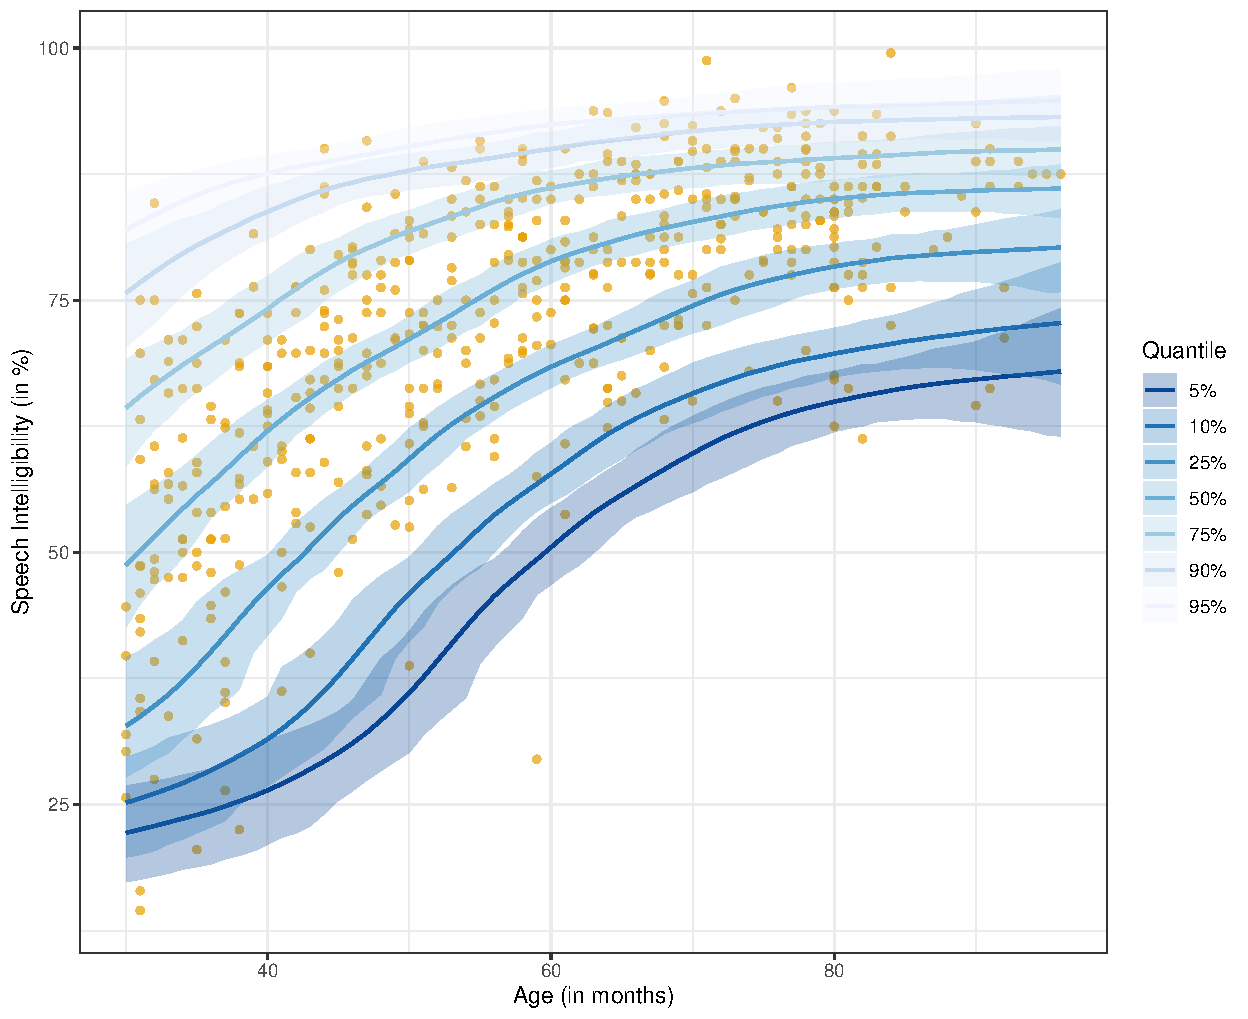
\includegraphics[width = 0.8\textwidth, height = 10cm]{plots/quantilesRDS3SingleWord.pdf}
    \caption{Quantile regression, $q_{\alpha}(\bx)$, with $90\%$ point-wise uncertainty intervals. $K = unif(z - c, z + c), \ c = 0.025$ and $G_0 = unif(0, 1)$. Intelligibility type: \textit{single-word}.}
    \label{fig:1}
\end{figure}

\begin{figure}[H]
    \centering
    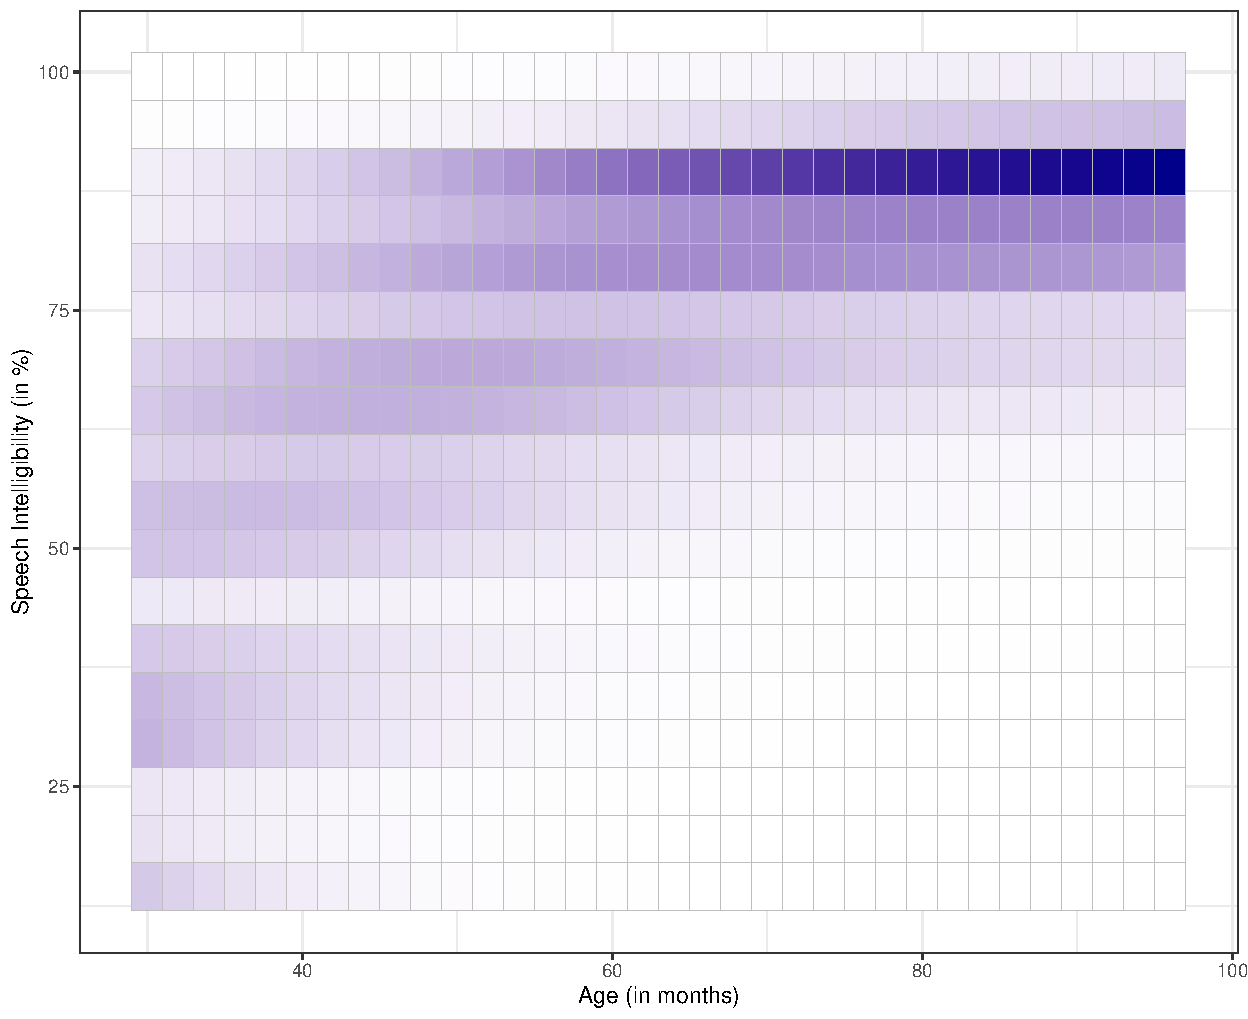
\includegraphics[width = 0.8\textwidth, height = 10cm]{plots/heatmapRDS3SingleWord.pdf}
    \caption{Heatmap for fitted probabilities, $\widehat p(y \mid x)$. $y$: Intelligibility (in $\%$) and $x$: Age (in months). Here `white' to `blue' represents an increase in $\widehat p(y \mid x)$. Intelligibility type: \textit{single-word}.}
    \label{fig:2}
\end{figure}

\begin{figure}[H]
    \centering
    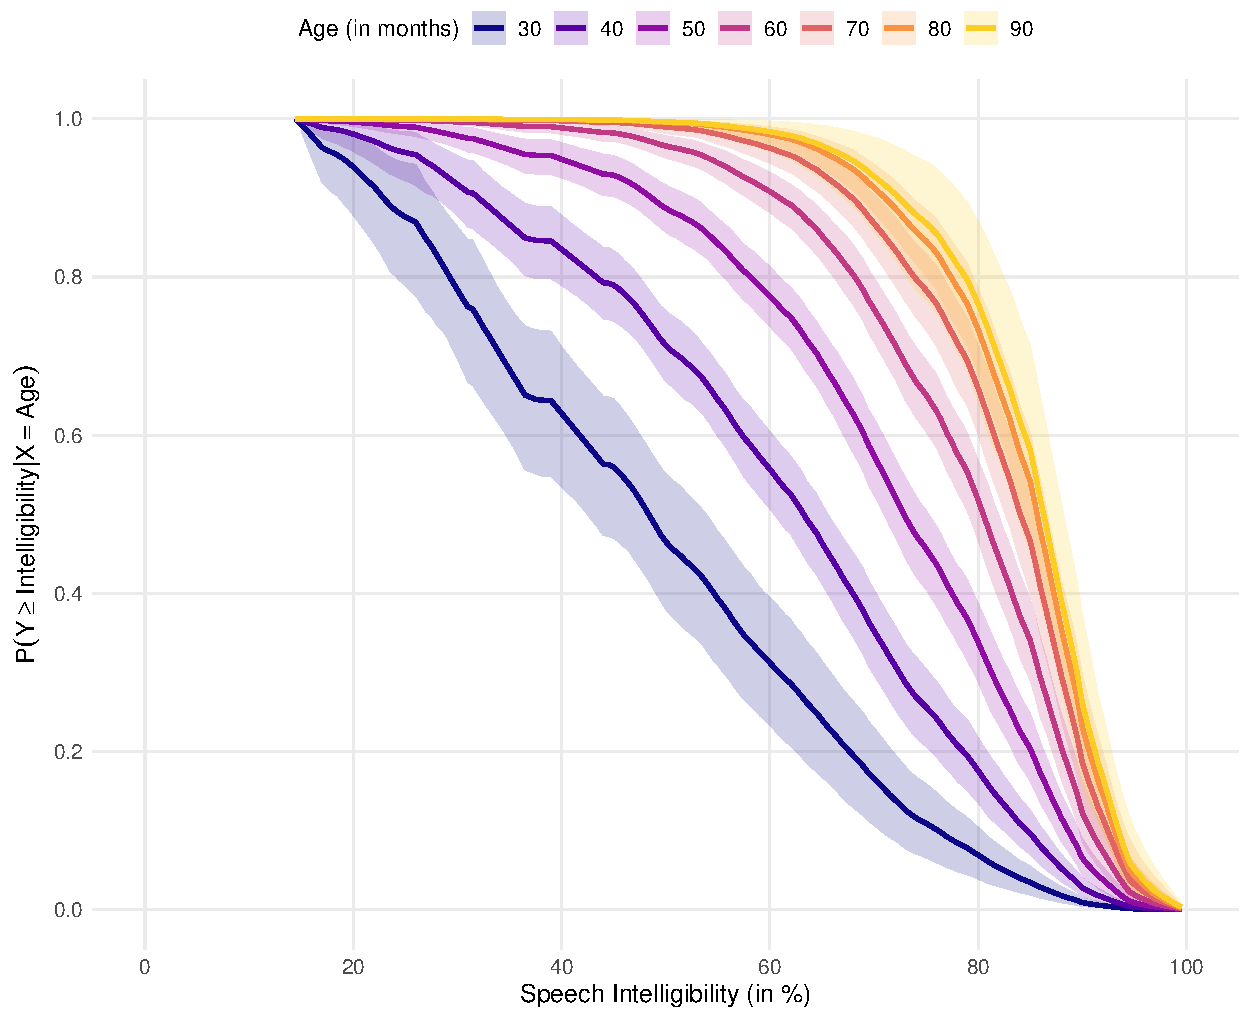
\includegraphics[width = 0.9\textwidth, height = 11cm]{plots/exceedanceRDS3SingleWord.pdf}
    \caption{Estimate for exceedance probabilities, $\widehat p(y \geq y_0 \mid x)$, with $90\%$ point-wise uncertainty intervals.. $y$: Intelligibility (in $\%$) and $x$: Age (in months). Intelligibility type: \textit{single-word}.}
    \label{fig:3}
\end{figure}


\subsection{%Inference for 
Study of multi word intelligibility}

\begin{figure}[H]
    \centering
    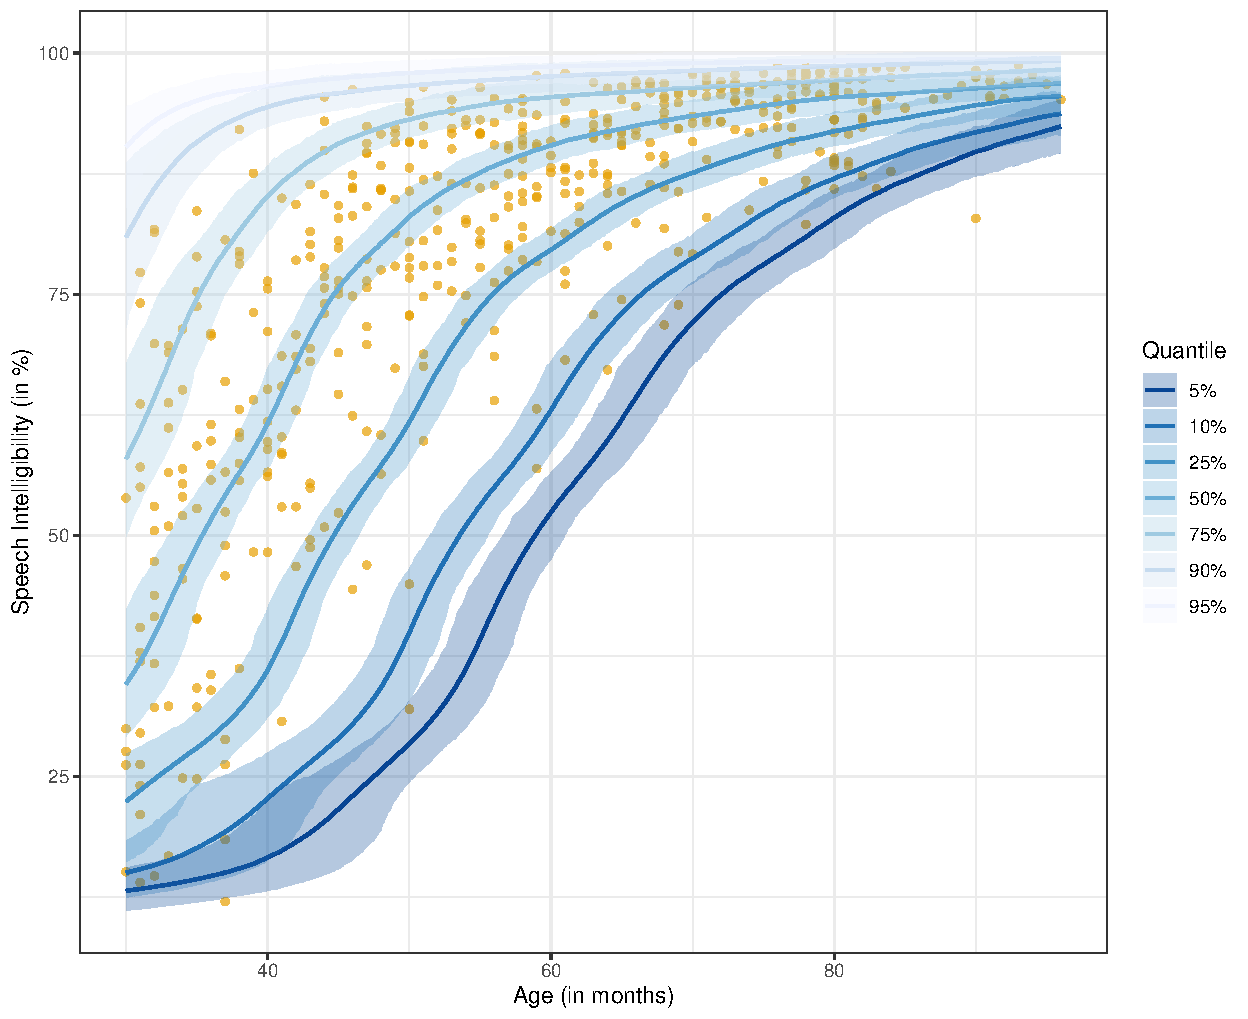
\includegraphics[width = 0.8\textwidth, height = 9.5cm]{plots/quantilesRDS3MultiWord.pdf}
    \caption{Quantile regression, $q_{\alpha}(\bx)$, with $90\%$ point-wise uncertainty intervals. $K = unif(z - c, z + c), \ c = 0.025$ and $G_0 = unif(0, 1)$. Intelligibility type: \textit{multi-word}.}
    \label{fig:4}
\end{figure}

\begin{figure}[H]
    \centering
    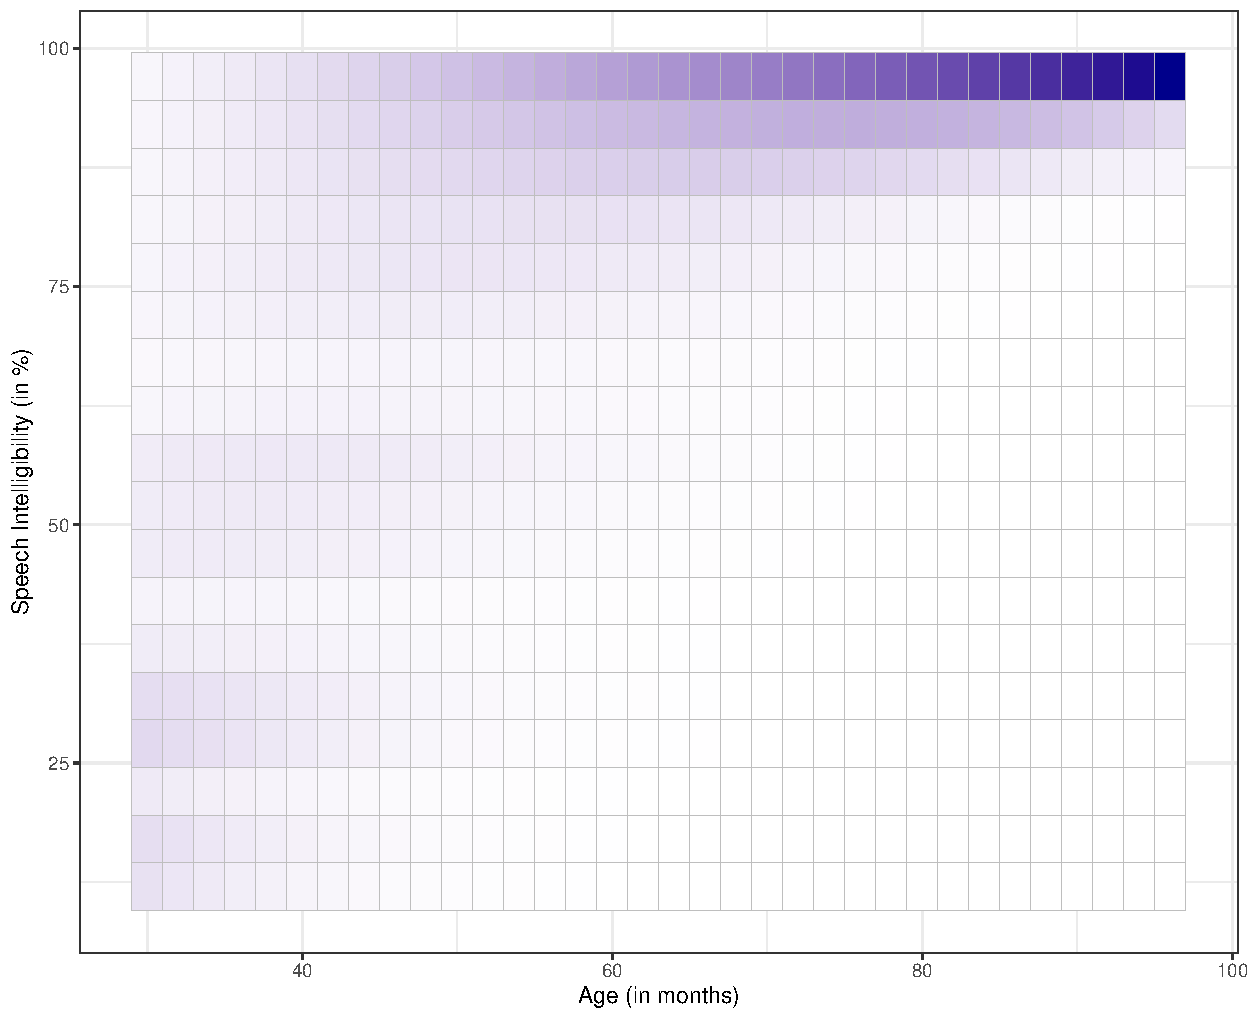
\includegraphics[width = 0.8\textwidth, height = 10cm]{plots/heatmapRDS3MultiWord.pdf}
    \caption{Heatmap for fitted probabilities, $\widehat p(y \mid x)$. $y$: Intelligibility (in $\%$) and $x$: Age (in months). Here `white' to `blue' represents an increase in $\widehat p(y \mid x)$. Intelligibility type: \textit{multi-word}.}
    \label{fig:5}
\end{figure}

\begin{figure}[H]
    \centering
    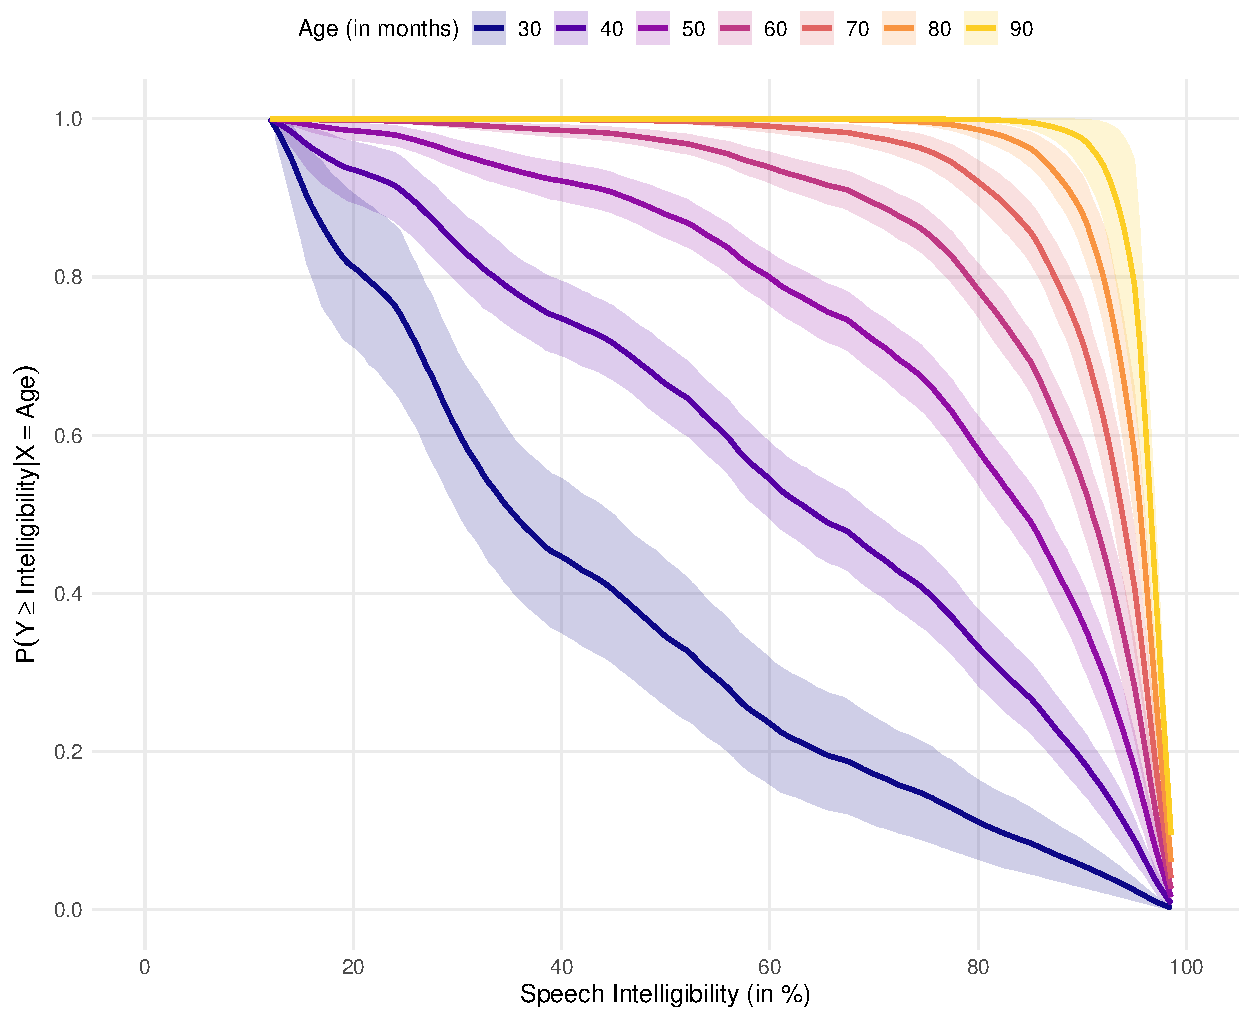
\includegraphics[width = 0.9\textwidth, height = 11cm]{plots/exceedanceRDS3MultiWord.pdf}
    \caption{Estimate for exceedance probabilities, $\widehat p(y \geq y_0 \mid x)$, with $90\%$ point-wise uncertainty intervals.. $y$: Intelligibility (in $\%$) and $x$: Age (in months). Intelligibility type: \textit{multi-word}.}
    \label{fig:6}
\end{figure}

\section{Discussion}
\label{sec:disc}

\section*{Supplementary Material}

\bibliography{references}

\subsubsection*{Acknowledgement}
Acknowledge Igor for Proposition 1.

\newpage 
\section*{Appendix}
% \subsection*{Proof of result 1}
% Let's assume that $\tilde{\mu}$ is a gamma completely random measure (CRM) with the base measure $G_0$ on the support $\YY$ and the concentration parameter $\alpha$. Therefore, we can express $\tilde{\mu}(\cdot)=\sum_{h=1}^{\infty} \omega_h \delta_{m_h}(\cdot)$ with the Levy intensity,
% $$
% \widetilde{\nu}(d y, d \omega)=\alpha \frac{e^{-\omega}}{\omega} d \omega G_0(d y)
% $$
% Therefore, we have $\tilde{\mu}(\YY) \sim Ga(\alpha G_0(\YY), 1) \equiv Ga(\alpha, 1)$, and we can write: $\frac{\tilde{\mu}}{\tilde{\mu}(\YY)} \sim DP(\alpha, G_0)$.

% \noindent Now, upon exponential tilting the $DP(\alpha, G_0)$, let's define a new CRM as follows:
% \begin{eqnarray*}
%   \tilde{\mu}^\star=\sum_{h=1}^{\infty} \omega^\star_h \delta_{m_h}, \mathrm{where} \ \omega^\star_h= \exp \left(\theta m_h\right) \omega_h  
% \end{eqnarray*}
% Now, using the Levy-Khintchine representation, for some measurable function $f$, the CRM $\tilde{\mu}^\star$ can be characterized by,
% \begin{eqnarray*}
% \E\left[e^{-\int_\YY f(y) \tilde{\mu}^\star(d y)}\right] & = & \E\left[e^{-\int_\YY f(y) \exp (\theta y) \mu(d y)} \right] \\
% & = & \E \left[e^{-\int_\YY g(y) \mu(d y)}\right] \\
% & & [\mathrm{define:} \ g(y) = \exp(\theta y) f(y) \mathrm{ \ is\ also\ a\ measurable\ function} ]\\
% & = & \exp \left\{-\int_{\RR^{+} \times \YY}\left[1-e^{-\omega g(y)}\right] \widetilde{\nu}(d y, d \omega)\right\} \\
% & = & \exp \left\{-\int_{\RR^{+} \times  \YY}\left[1-e^{-\omega f(y) \exp (\theta y)}\right] \alpha \frac{e^{-\omega}}{\omega} d \omega G_0(dy)\right\}\\
% & = & \exp \left\{-\int_{\RR^{+} \times  \YY}\left[1-e^{-\omega^\star f(y)}\right] \alpha \frac{e^{-\omega^\star/\exp(\theta y)}}{\omega^\star} d \omega^\star G_0(dy)\right\} \\
% & & \left[\mathrm{using \ change \ of \ variable:} \ \omega^\star = \omega \exp(\theta y)\right]
% \end{eqnarray*}
% Hence, we can say that the exponentially tilted CRM $\tilde{\mu}^\star$ has the Levy intensity,
% $$
% \nu(d y, d \omega)=\alpha \cdot \frac{e^{- \omega / \exp (\theta y)}}{\omega} d\omega G_0(dy)
% $$
\end{document}

